\subsection{Front-end module architecture}
In this section is shown how the Front-end module of EmporioLambda works. In particular it will be explained the role of every part of it.\\The Front-end module can be summarized in 4 primary parts:
\begin{itemize}
\item data pre-fetching: managed with Next.js;
\item components: managed with React;
\item services: functions that communicate with Back-end module;
\item types: classes and data types used.
\end{itemize} 
How these parts communicate each other is illustrated in the image below:
\begin{figure}[H]
\centering
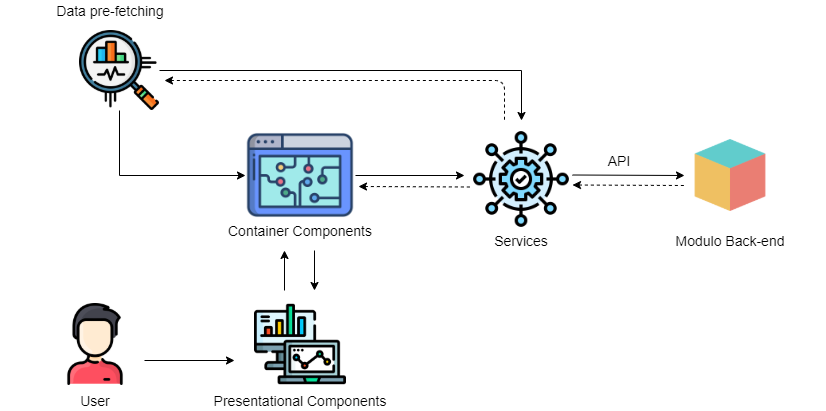
\includegraphics[scale=0.58]{res/Architettura/Frontend/img/general_frontend}\\
\caption{Front-end module general scheme}
\end{figure}


